% Part 1 report (02.11.2026 - 30.11.2026). Compile from this folder:
%   pdflatex -interaction=nonstopmode progress-report-01.tex   (twice, for references)
\documentclass[runningheads]{llncs}

\usepackage[T1]{fontenc}
\usepackage[utf8]{inputenc}
\usepackage{graphicx}
\usepackage{float}
\usepackage{amsmath}
\usepackage{booktabs}
\usepackage{url}
\usepackage{cite}
\usepackage{caption}
\captionsetup{font=small}

\begin{document}

\title{Development of GrowingNN Architecture Search Algorithms in PyTorch\\
Results Report, Part 1 (02.11.2026 -- 30.11.2026)\thanks{This work was carried out under agreement no.~UMO-2024/53/B/ST6/00021 with the National Science Centre, Poland (Narodowe Centrum Nauki).}}
\titlerunning{GrowingNN Architecture Search -- Part 1}
\author{Szymon Świderski}
\authorrunning{S. Świderski}
\institute{}
\maketitle

\begin{abstract}
This report presents the experiments that turned the PyTorch implementation of GrowingNN into a working architecture-growth method. GrowingNN trains a network in generations and, between them, a search algorithm chooses one change to its architecture. On MNIST we decided when the search should run, which starting networks it can grow, and which search algorithms to keep, comparing thirteen of them over 130 runs. On CIFAR-10 the first runs either stopped learning near 67\% or memorized the training set; after changes to augmentation, the learning rate and the way new convolutions are inserted, the grown networks kept learning across generations and three runs finished at 91.11\%, 91.17\% and 91.36\% official test accuracy. With all actions available to the search, the method reached 96.3\% on MNIST, 86.4\% on CIFAR-10 and 62.8\% on CIFAR-100, with networks 3 to 10 times smaller than standard reference models.
\keywords{dynamic neural networks \and neural architecture search \and Monte Carlo tree search \and CIFAR-10}
\end{abstract}

\section{Introduction}

GrowingNN~\cite{growingnn_original} trains a neural network in \emph{generations}. After each generation a search algorithm may apply one change to the architecture, for example adding a convolution or a residual branch, and training continues with the changed network. To choose the change, the search briefly trains a copy of the network with each candidate change on a small \emph{simulation set} and compares the results. The earlier implementation reports described how these actions and the training loop were rebuilt in PyTorch with \texttt{torch.fx}. This report presents the experiments that tuned and tested the search.

Three accuracies are used. \emph{Training accuracy} is measured on the images used to update the weights, \emph{validation accuracy} on held-out images that the search may use, and \emph{official test accuracy} on the separate CIFAR test set of 10{,}000 images, which the search never sees.

\section{When and What the Search Can Change (MNIST)}

All MNIST runs start from a very small convolutional network of a few hundred parameters, so the search has to build most of the network itself.

\subsection{When the search runs}

Running the search while the network is still learning quickly wastes the gain of the current architecture. A \emph{slope threshold} lets the search run only when the training curve has flattened, and after each change the learning rate warms up again to its target. Experiment 000 compared two thresholds and three warm-up curves (Fig.~\ref{fig:000}).

\begin{figure}[!htbp]
\centering
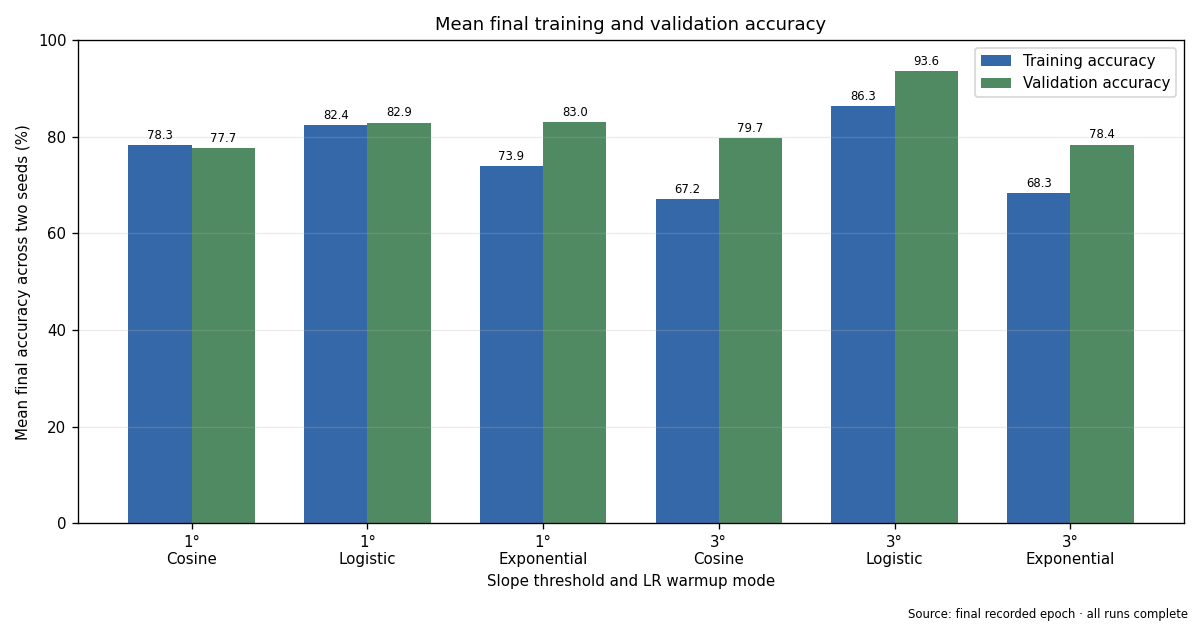
\includegraphics[width=0.78\textwidth]{figures/000-final-accuracy.png}
\caption{When to search: mean final training (blue) and validation (green) accuracy for each slope threshold and warm-up curve, two seeds each.}
\label{fig:000}
\end{figure}

A \(3^\circ\) threshold with a logistic warm-up was clearly best, at 93.6\% validation against 77.7--83.0\% for the other pairs. Most of the gain came from the first architecture change, and residual convolutions were the most useful action.

\subsection{Which networks the search can grow}

With the \(3^\circ\) setting, three starting depths were compared. The largest starter ended at 91.2\% validation and the smallest at only 48.9\% (Fig.~\ref{fig:001}). The action records showed why: no sequential convolution could ever be inserted on these graphs, so a thin network had no direct way to rebuild a missing convolution, and the search instead spent generations adding and deleting layers.

\begin{figure}[!htbp]
\centering
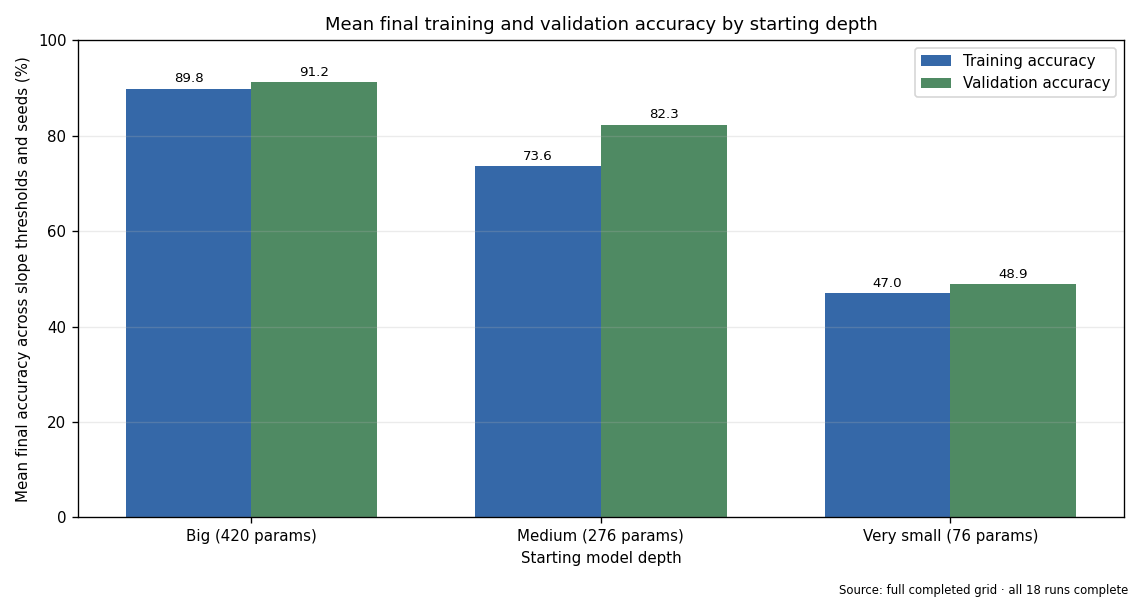
\includegraphics[width=0.7\textwidth]{figures/001-final-accuracy.png}
\caption{Starting depth: mean final accuracy for the big, medium and very small starters.}
\label{fig:001}
\end{figure}

After sequential convolutions could be inserted before the classifier, even the small starter could grow into a deeper convolutional network by itself (Fig.~\ref{fig:002}).

\begin{figure}[!htbp]
\centering
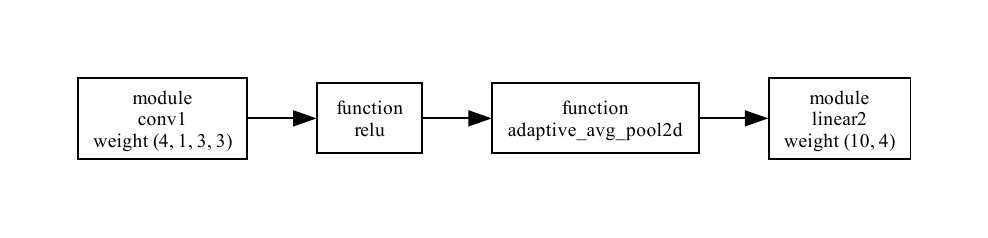
\includegraphics[width=0.5\textwidth]{figures/002-start-small.png}\\[2mm]
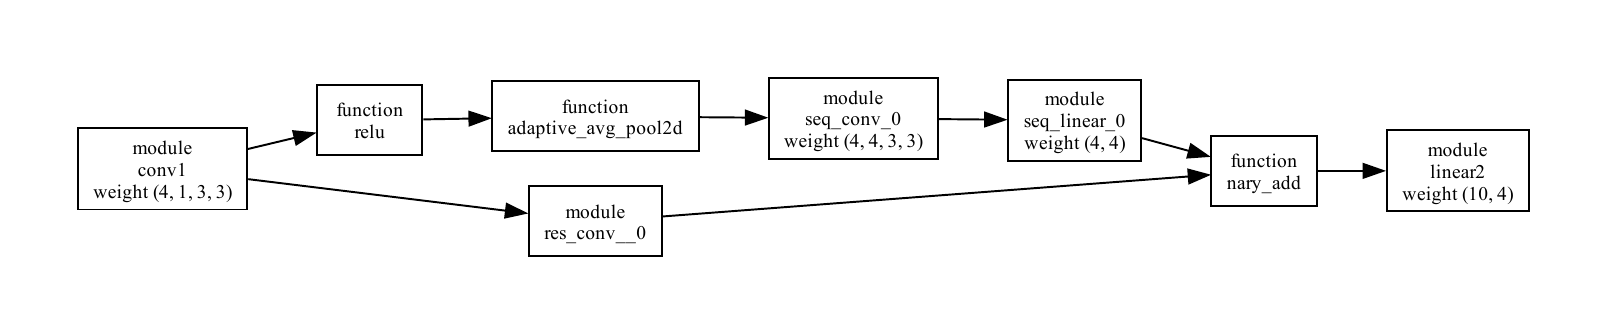
\includegraphics[width=0.95\textwidth]{figures/002-final-small.png}
\caption{The small starter (top) and the network the search grew from it in five generations (bottom, 62\% validation), drawn from the run's graph.}
\label{fig:002}
\end{figure}

\subsection{Which search algorithm to keep}

The original search is Monte Carlo tree search (MCTS). It can look several changes ahead, but its results varied strongly between seeds. Thirteen search algorithms were compared on two starters with five seeds each, 130 runs in total (Fig.~\ref{fig:005}).

\begin{figure}[!htbp]
\centering
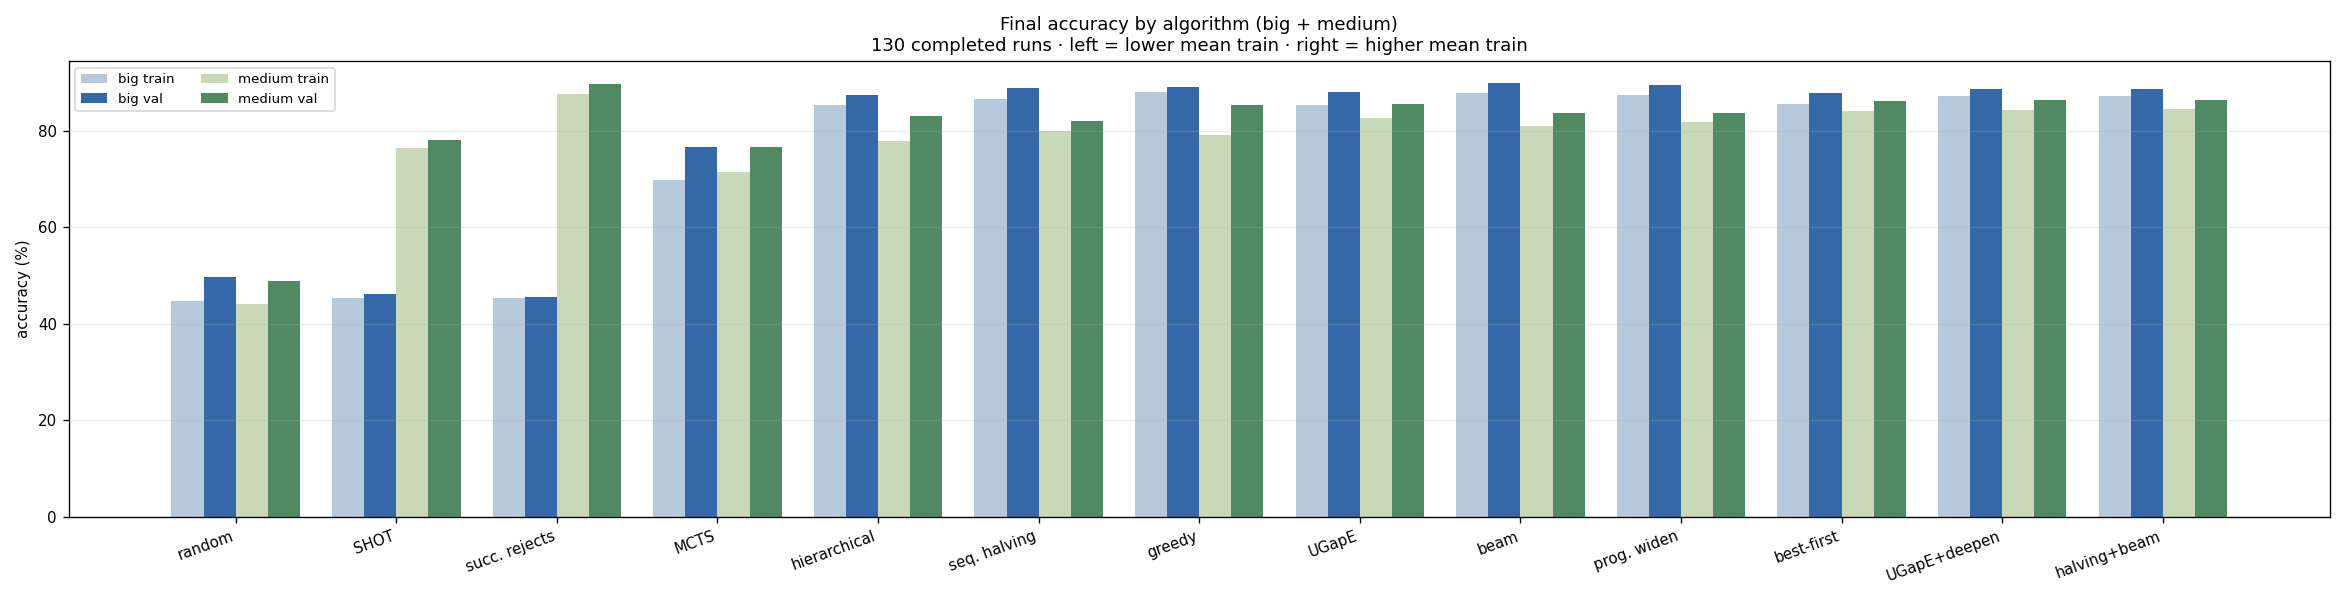
\includegraphics[width=\textwidth]{figures/005-final-accuracy-combined.png}
\caption{Search algorithms: final training and validation accuracy for each algorithm, on the big and medium starters.}
\label{fig:005}
\end{figure}

Four look-ahead algorithms were kept: sequential halving with a beam, UGapE with deepening, best-first search and beam search. MCTS, greedy and random search remained as references, and six algorithms were dropped. MNIST turned out to be easy: greedy search was already near the top, so this comparison was a filter before harder tasks, not a final ranking.

\section{Making Growth Work on CIFAR-10}

\subsection{The problem: the network stalls or memorizes}

On CIFAR-10 the method at first did not keep learning. With live augmentation (random crop and flip), ten generations of 100 epochs flattened near 67\% test accuracy (Fig.~\ref{fig:early}, top). Without augmentation the network reached 98\% training accuracy while test accuracy fell to 45\%: it memorized the training images (Fig.~\ref{fig:early}, bottom). Across 24 runs of 400 epochs, augmentation raised the mean final test accuracy from 65.6\% to 77.0\%, so it was kept.

\begin{figure}[!htbp]
\centering
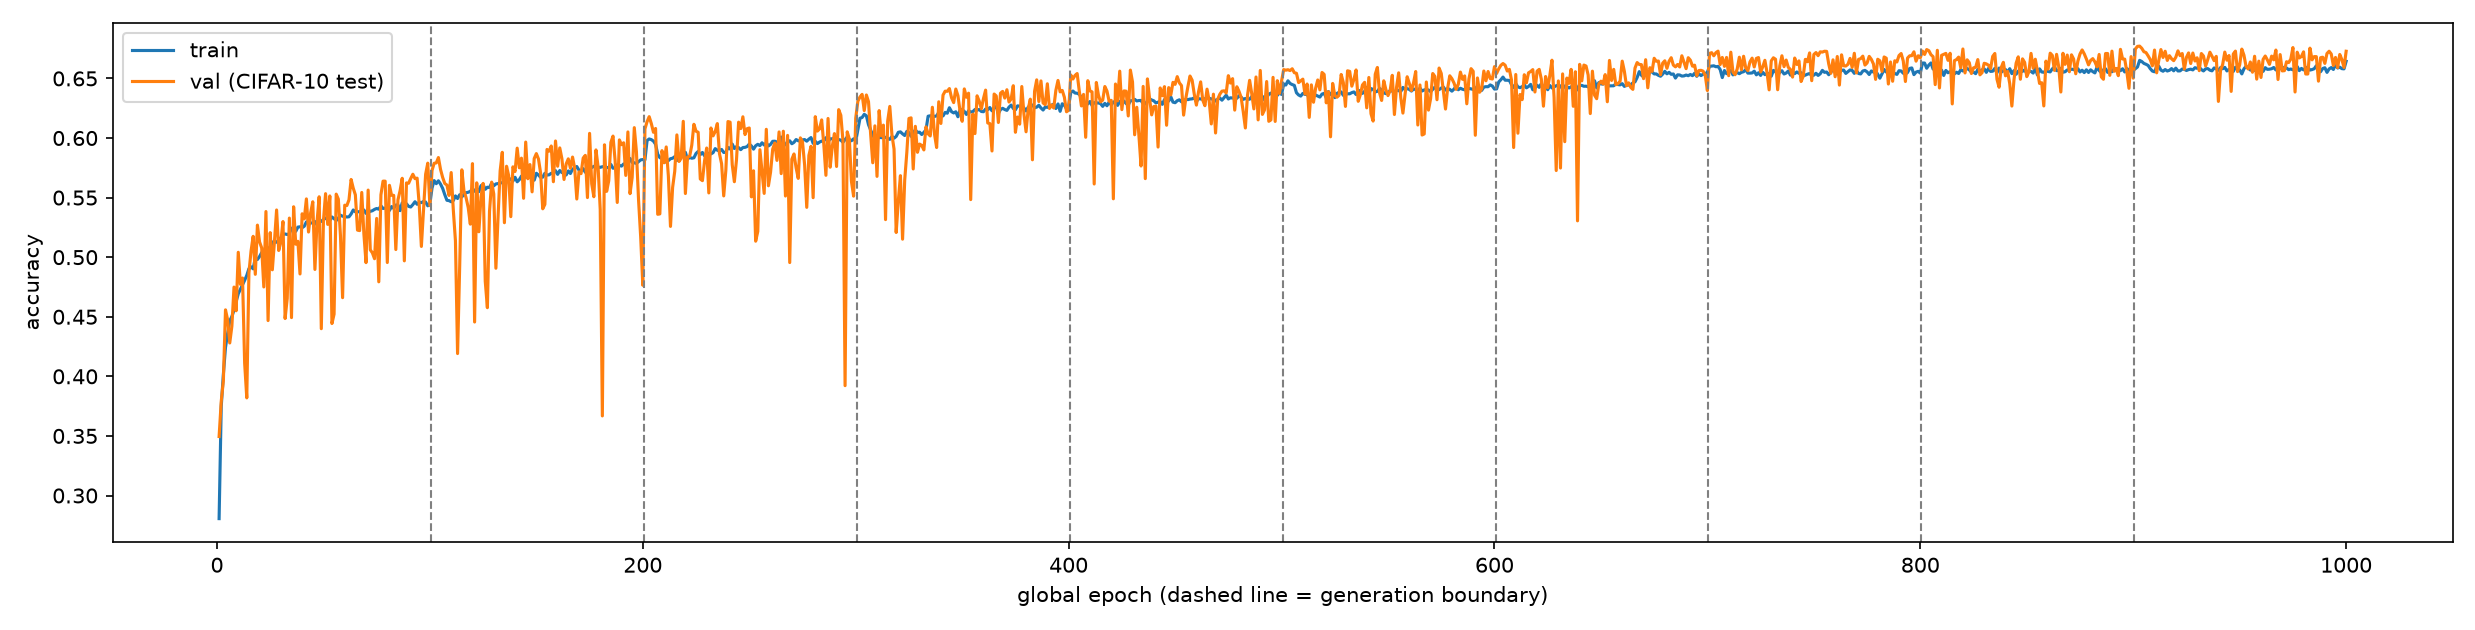
\includegraphics[width=\textwidth]{figures/cifar-summary-early-augmented.png}\\[1mm]
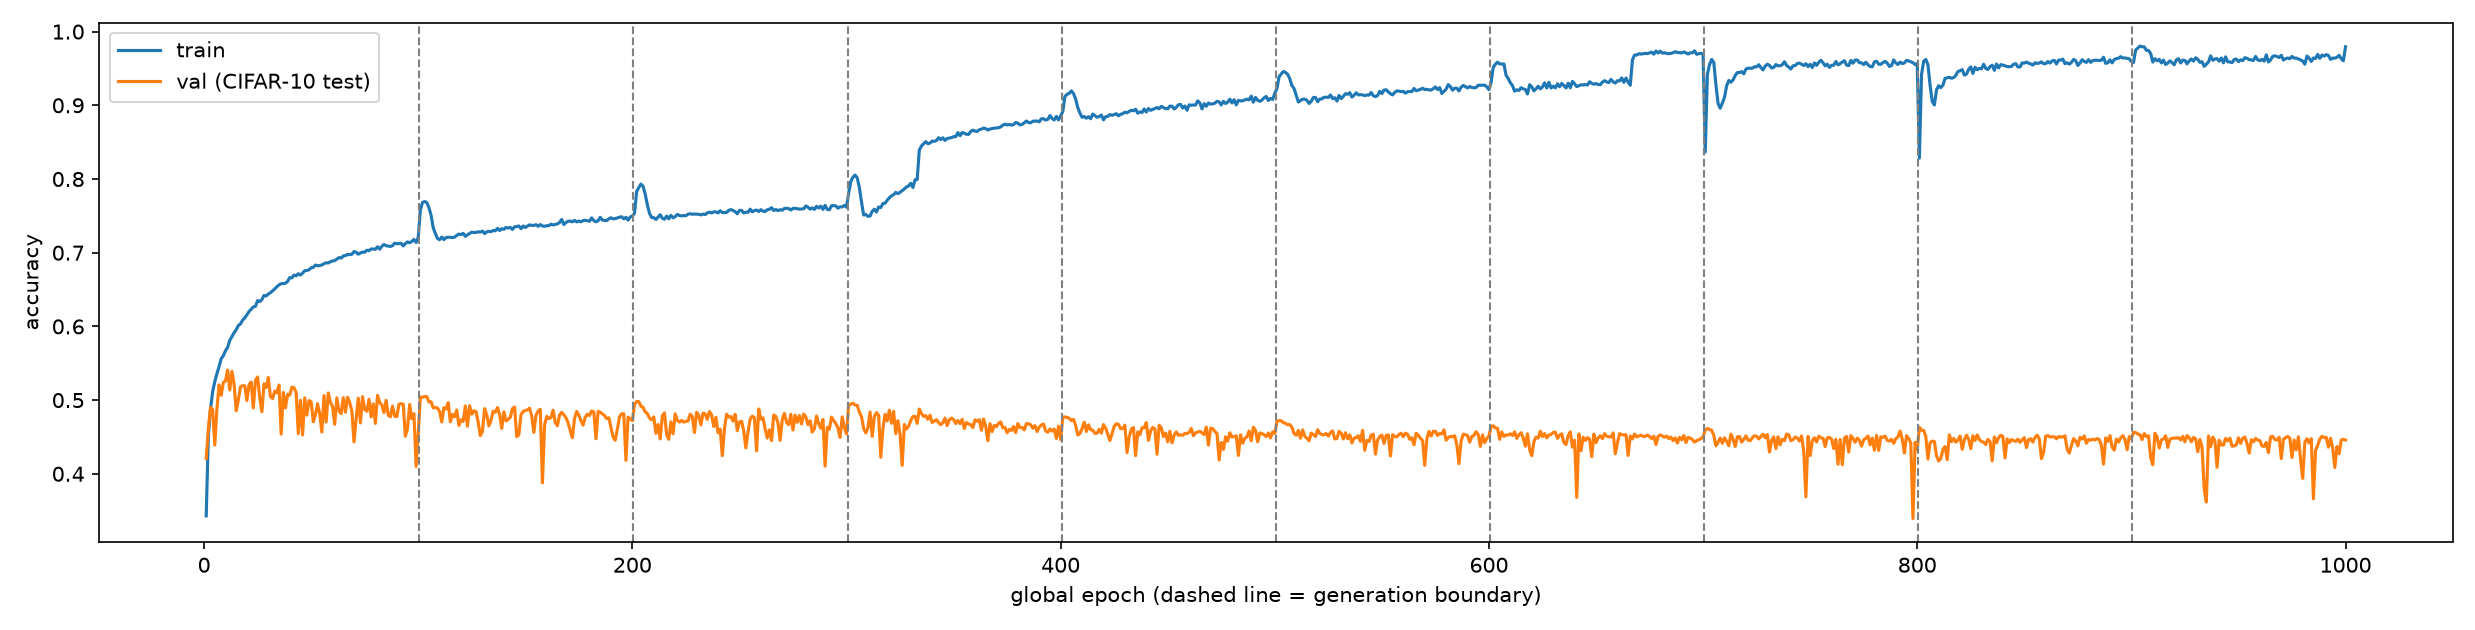
\includegraphics[width=\textwidth]{figures/cifar-summary-early-no-augmentation.png}
\caption{Early CIFAR-10 runs, 10 generations of 100 epochs. Top: with live augmentation both curves flatten near 67\%. Bottom: without it training reaches 98\% while test falls to 45\%.}
\label{fig:early}
\end{figure}

\subsection{A better network exists}

A slow diagnostic search trained every candidate for 100 epochs on the full training set. It found a sequence of six convolution widenings that raised test accuracy from 57.9\% to 80.3\% (Fig.~\ref{fig:widening}). The small starter could therefore become a good network; the cheap search simply did not find this path, and the training setup did not let the grown networks learn enough.

\begin{figure}[!htbp]
\centering
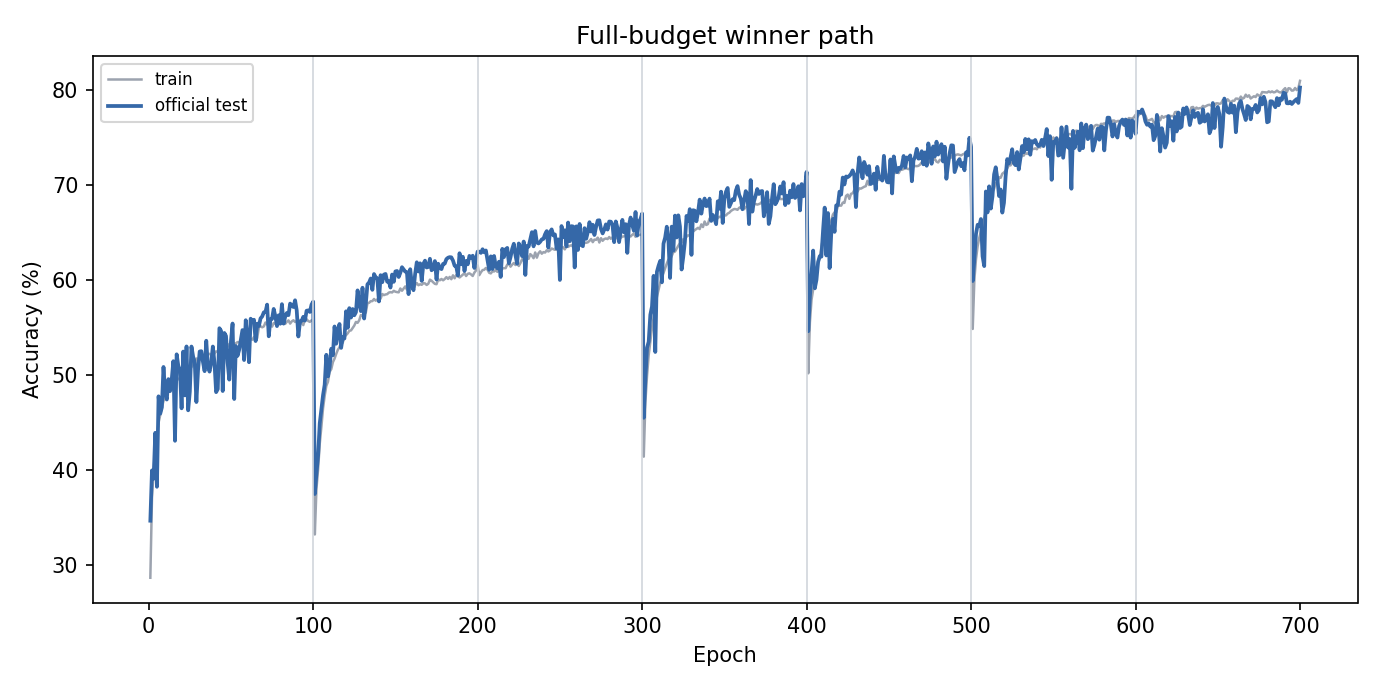
\includegraphics[width=0.7\textwidth]{figures/cifar-summary-manual-widening.png}
\caption{Diagnostic search with full training of each candidate: each kept widening raises test accuracy further.}
\label{fig:widening}
\end{figure}

\subsection{What made the grown network learn}

Two changes were tested separately and together with five seeds: a global learning rate from 0.1 to 0.001 that is not restarted after each change, and inserting new convolutions before global pooling, on an \(8\times8\) map, with BatchNorm and ReLU, instead of after pooling. Each change alone gave about 83\% test; together they reached 88.0\% (Fig.~\ref{fig:lrconv}). With these changes, a wider starter with BatchNorm and ten training epochs per generation, the search could keep improving the network.

\begin{figure}[!htbp]
\centering
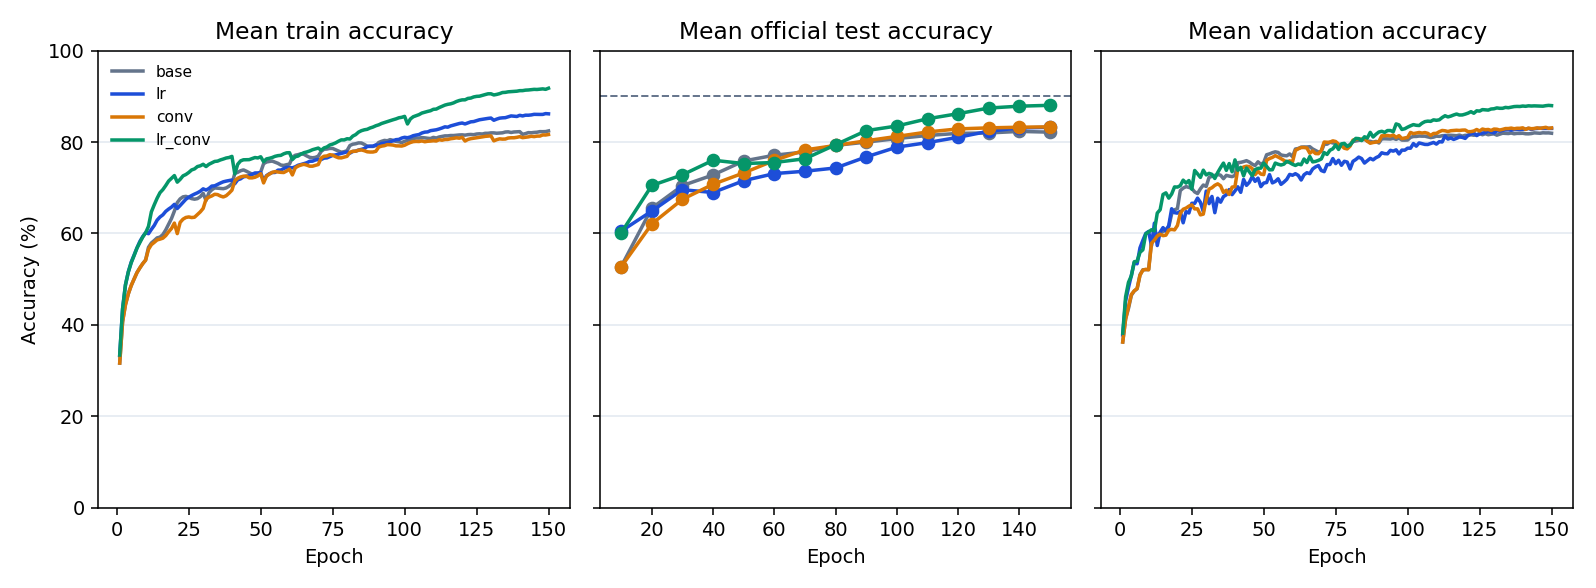
\includegraphics[width=\textwidth]{figures/cifar-summary-training-convolution-histories.png}
\caption{Five-seed mean training, official test and validation. Green combines the new learning rate and the new convolution insertion; gray changes neither, blue only the learning rate, orange only the convolution.}
\label{fig:lrconv}
\end{figure}

\subsection{Result: learning continues across generations}

With every action available to the search and 15 generations of 10 epochs, all three seeds reached about 90\% official test, 90.04\% on average (Fig.~\ref{fig:gencount}). The most consistent configuration let the search add only sequential convolutions: all three seeds passed 90\% before the last generation and finished at their best value (Fig.~\ref{fig:reference}, Table~\ref{tab:reference}), with training, validation and test rising together. The network grew from 187{,}008 to 1.8 million parameters.

\begin{figure}[!htbp]
\centering
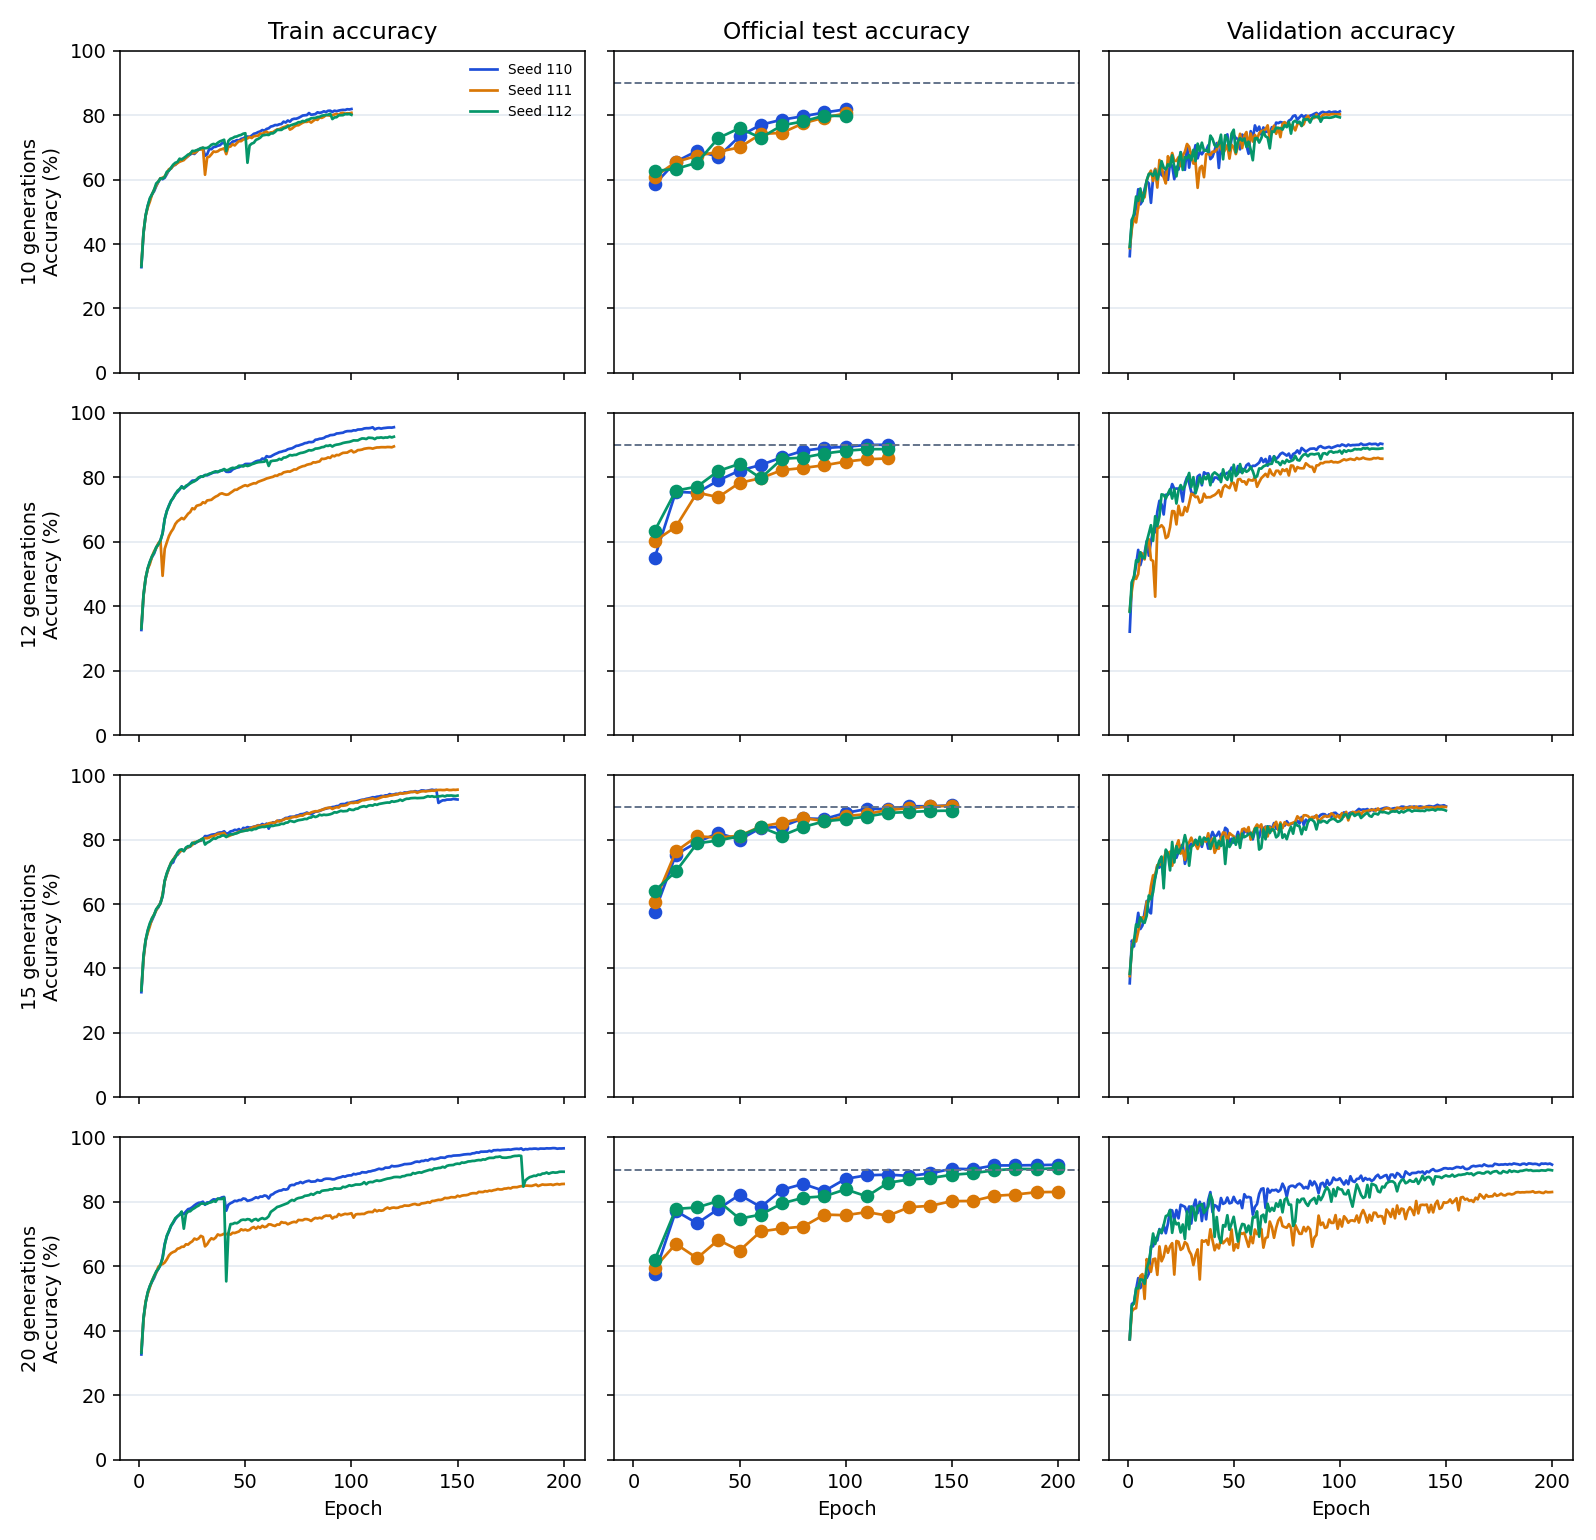
\includegraphics[width=0.75\textwidth]{figures/cifar-summary-generation-count-histories.png}
\caption{All actions available, 10, 12, 15 and 20 generations (rows): training, official test and validation, three seeds each. With 15 generations every seed reaches about 90\%.}
\label{fig:gencount}
\end{figure}

\begin{figure}[!htbp]
\centering
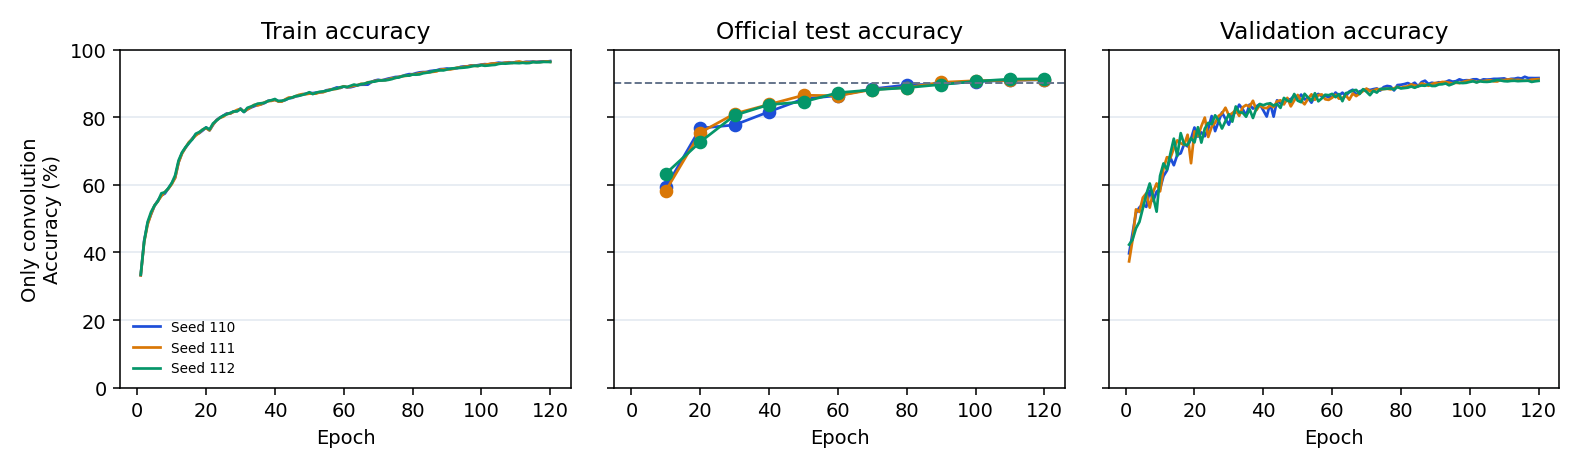
\includegraphics[width=\textwidth]{figures/cifar-summary-final-training-curves.png}
\caption{Growth by sequential convolutions, 12 generations of 10 epochs: training (left), official test (middle) and validation (right) for three seeds.}
\label{fig:reference}
\end{figure}

\begin{table}[!htbp]
\centering
\caption{Official test accuracy of the sequential-convolution runs at the end of selected generations.}
\label{tab:reference}
\begin{tabular}{rrrrr}
\toprule
Epoch & Seed 110 & Seed 111 & Seed 112 & Mean \\
\midrule
10 & 59.27\% & 58.32\% & 63.35\% & 60.31\% \\
40 & 81.65\% & 83.80\% & 83.74\% & 83.06\% \\
100 & 90.55\% & 90.82\% & 90.64\% & 90.67\% \\
120 & \textbf{91.11\%} & \textbf{91.17\%} & \textbf{91.36\%} & \textbf{91.21\%} \\
\bottomrule
\end{tabular}
\end{table}

\section{Three Datasets}

Finally, the method ran with every action available for 20 generations of 10 epochs on MNIST, CIFAR-10 and CIFAR-100, three seeds each (Fig.~\ref{fig:009}, Table~\ref{tab:009}).

\begin{figure}[!htbp]
\centering
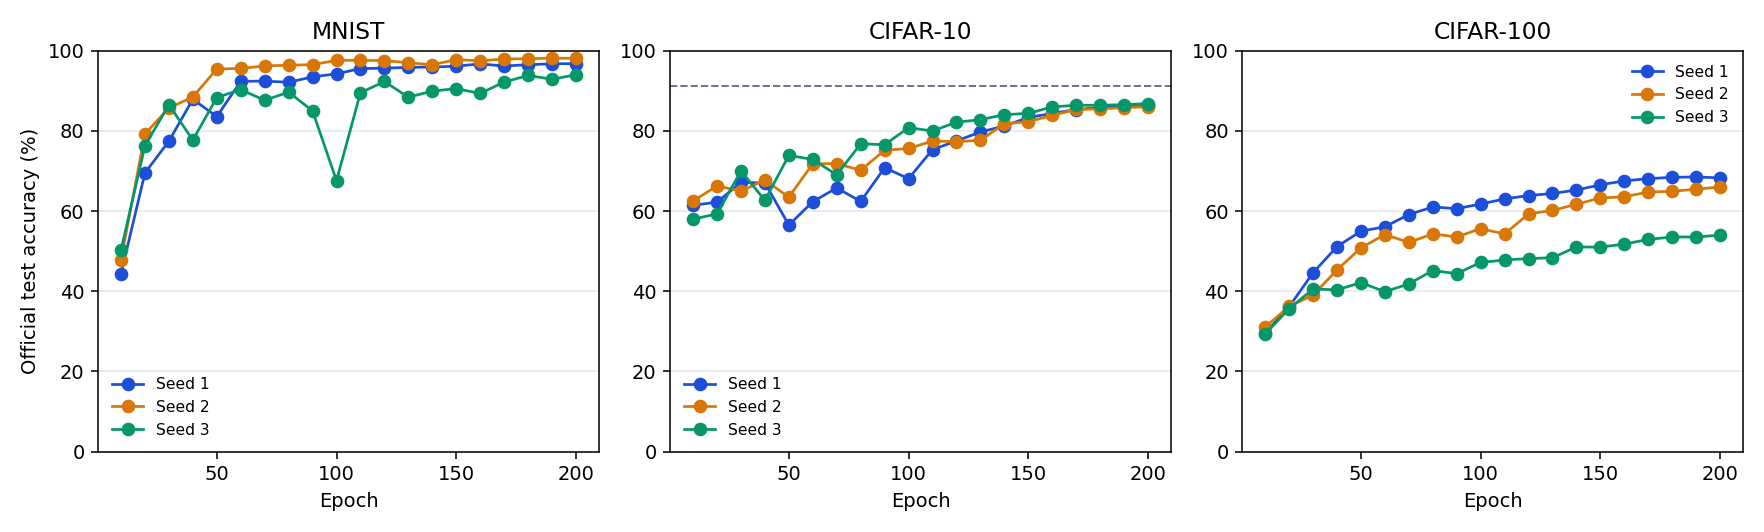
\includegraphics[width=\textwidth]{figures/009-small20-test-by-generation.png}
\caption{Official test accuracy after each generation on the three datasets; colors are seeds. The dashed CIFAR-10 line is the 91.21\% sequential-convolution result.}
\label{fig:009}
\end{figure}

\begin{table}[!htbp]
\centering
\caption{Final official test accuracy and size of the grown networks.}
\label{tab:009}
\begin{tabular}{lrrrrl}
\toprule
Dataset & Seed 1 & Seed 2 & Seed 3 & Mean & Parameters \\
\midrule
MNIST & 96.77\% & 98.09\% & 93.99\% & 96.28\% & 5.8--9.0 k \\
CIFAR-10 & 86.25\% & 86.04\% & 86.82\% & 86.37\% & 1.5--2.2 M \\
CIFAR-100 & 68.26\% & 66.02\% & 54.00\% & 62.76\% & 1.8--3.9 M \\
\bottomrule
\end{tabular}
\end{table}

CIFAR-10 was stable across seeds, with a spread of 0.78 points. All grown networks are smaller than standard references: 6 to 11 times smaller than LeNet-5 on MNIST and 3 to 7 times smaller than ResNet-18 on CIFAR. Fig.~\ref{fig:009-actions} shows which actions the search chose and what followed: sequential convolutions gave the largest gains, while on CIFAR-10 the search mostly added residual linear layers, which explains why it stayed below the sequential-convolution result.

\begin{figure}[!htbp]
\centering
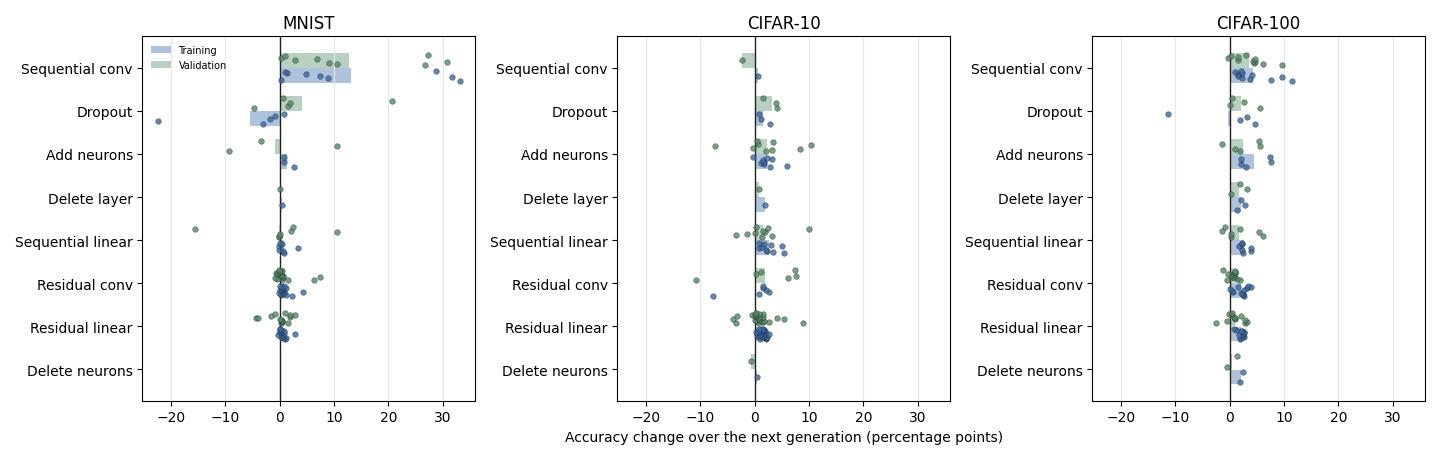
\includegraphics[width=\textwidth]{figures/009-small20-action-types-by-dataset.png}
\caption{Change in training (blue) and validation (green) accuracy over the generation after each action, by action type and dataset.}
\label{fig:009-actions}
\end{figure}

\section{Summary}

The search in the PyTorch implementation of GrowingNN now grows networks that keep learning: on CIFAR-10 the grown networks finished above 91\% official test on all three seeds, up from runs that stalled near 67\% or memorized the training set. On MNIST we fixed when the search runs (a \(3^\circ\) slope threshold with logistic warm-up), made sequential convolutions available so that small networks can grow, and selected four look-ahead search algorithms with MCTS as reference. With every action available, the method reached 96.3\%, 86.4\% and 62.8\% on MNIST, CIFAR-10 and CIFAR-100 with compact networks.

Two limits remain. The best result restricts the search to one action type; with all actions available, it sometimes chooses changes that slow learning. How the search grades candidates, and which images it uses for that, is therefore the subject of the next part of the work.

\subsubsection*{Acknowledgments.} The results presented in this report were obtained under agreement no.~UMO-2024/53/B/ST6/00021 with the National Science Centre, Poland (Narodowe Centrum Nauki, NCN).

\begin{thebibliography}{1}
\bibitem{growingnn_original}
Świderski, S., Jastrzębska, A.: Dynamic Growing and Shrinking of Neural Networks with Monte Carlo Tree Search. In: Computational Science -- ICCS 2024. LNCS, vol. 14832. Springer (2024). \url{https://doi.org/10.1007/978-3-031-63749-0_25}
\end{thebibliography}

\end{document}
